\documentclass{article}
\usepackage[final]{neurips_2020}
\usepackage[utf8]{inputenc}
\usepackage{ctex}
\usepackage[T1]{fontenc}
\usepackage{hyperref}
\usepackage{url}
\usepackage{booktabs}
\usepackage{algorithm}
\usepackage{algpseudocode}  % 这个包用于算法伪代码

\usepackage{amsfonts}
\usepackage{amsmath}
\usepackage{nicefrac}
\usepackage{microtype}
\usepackage{indentfirst}
\usepackage{listings}
\usepackage{graphicx}
\usepackage{float}
\usepackage{media9}

\usepackage[dvipsnames]{xcolor}
\lstset{
    language=Python,
    basicstyle=\ttfamily,
    breaklines=true,
    keywordstyle=\bfseries\color{NavyBlue},
    morekeywords={},
    emph={self},
    emphstyle=\bfseries\color{Rhodamine},
    commentstyle=\itshape\color{black!50!white},
    stringstyle=\bfseries\color{PineGreen!90!black},
    columns=flexible,
    numbers=left,
    numbersep=2em,
    numberstyle=\footnotesize,
    frame=single,
    framesep=1em,
    showstringspaces=false
}
\setlength{\parindent}{2em}

\title{中山大学计算机院本科生实验报告\\
    (2024学年秋季学期)}

\begin{document}
\maketitle
课程名称:强化学习与博弈论 \qquad\qquad\qquad\qquad\qquad\qquad
批改人:
\begin{table*}[h]
    \centering
    \begin{tabular}{|c|c|c|c|} \hline
        实验    & Assignment3                 & 专业(方向) & 计算机科学与技术 计科一班 \\ \hline
        学号    & 21307099                           & 姓名     & 李英骏           \\\hline
        Email & \texttt{liyj323@mail2.sysu.edu.cn} & 完成日期   & \today        \\\hline
    \end{tabular}
\end{table*}
\tableofcontents

\newpage

\section{应用案例说明}
CarRacing是OpenAI Gym提供的一个经典强化学习环境,用于测试智能体在连续动作空间中控制车辆的能力。本实验使用DQN(Deep Q-Network)算法解决该问题,训练智能体使其能够在给定赛道上尽可能长时间保持行驶并获得高分。

\section{算法实现核心思路}
DQN算法结合了深度学习和强化学习的思想,通过卷积神经网络(CNN)近似动作值函数(Q函数)。

\subsection{算法公式}
DQN的核心公式如下:
\begin{equation}
Q(s_t, a_t; \theta) = r_t + \gamma \max_{a'} Q(s_{t+1}, a'; \theta^-),
\end{equation}
其中:
\begin{itemize}
    \item $s_t$ 和 $s_{t+1}$ 分别表示当前状态和下一状态;
    \item $a_t$ 和 $a'$ 分别表示当前动作和下一动作;
    \item $r_t$ 表示即时奖励;
    \item $\gamma$ 为折扣因子,控制未来奖励的权重;
    \item $\theta$ 和 $\theta^-$ 分别表示当前网络和目标网络的参数。
\end{itemize}

目标是通过最小化均方误差(MSE)优化网络参数:
\begin{equation}
L(\theta) = \mathbb{E}\big[ (y_t - Q(s_t, a_t; \theta))^2 \big],
\end{equation}
其中:
\begin{equation}
y_t = r_t + \gamma \max_{a'} Q(s_{t+1}, a'; \theta^-).
\end{equation}

\subsection{算法伪代码}
以下为DQN的核心伪代码:
\begin{verbatim}
Initialize policy network Q with weights \theta
Initialize target network Q' with weights \theta^- = \theta
Initialize replay buffer D

for episode in num_episodes do
    Initialize state s
    for step in max_steps do
        With probability \epsilon select a random action a
        Otherwise select a = argmax Q(s, a; \theta)
        Execute action a, observe reward r and next state s'
        Store (s, a, r, s') in replay buffer D
        Sample random mini-batch from D
        Compute target y and loss L
        Perform gradient descent to update \theta
        Update target network \theta^- periodically
    end for
end for
\end{verbatim}

\section{实验结果及分析}

\subsection{训练曲线}
在训练过程中,我们记录了每一回合的总奖励(Reward)。如图\ref{fig:training_curve}所示,随着训练的进行,智能体的表现逐渐提升。

\begin{figure}[h!]
    \centering
    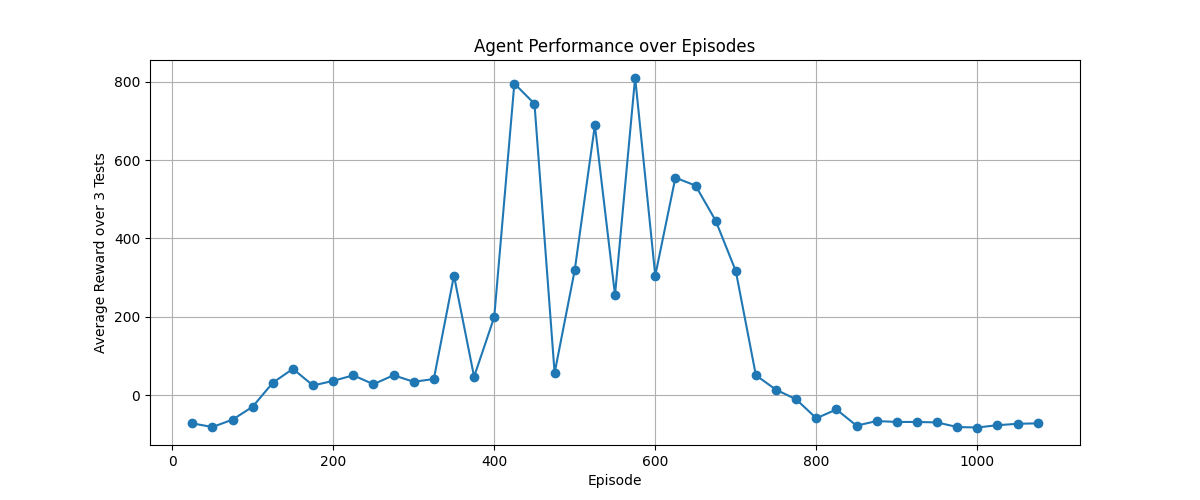
\includegraphics[width=0.8\textwidth]{./image/Figure_1.png}
    \caption{训练过程中每回合的奖励曲线}
    \label{fig:training_curve}
\end{figure}

\subsection{测试表现}
在测试阶段,使用训练好的模型对智能体进行评估。下图\ref{fig:car_racing_example}展示了智能体在CarRacing环境中的表现。
\begin{figure}[h!]
    \centering
    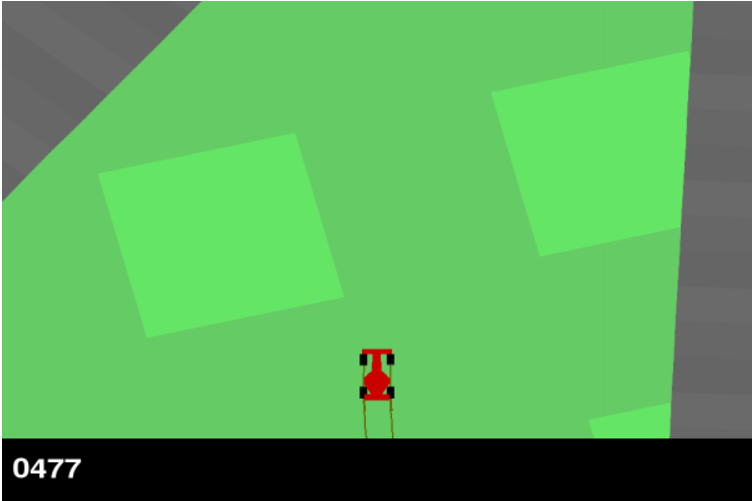
\includegraphics[width=0.8\textwidth]{./image/Figure_2.png}
    \caption{训练过程中每回合的奖励曲线}
    \label{fig:car_racing_example}
\end{figure}

\subsection{GIF生成}
我们进一步生成了智能体在测试过程中的行为\href{https://github.com/KFCCrazzzyThursday/rl_and_game_theory/blob/main/car_racing.gif}{GIF},用于直观地展示智能体的表现。
\section{结论}
本实验通过DQN算法成功训练了一个能够在CarRacing环境中表现良好的智能体。实验结果表明:
\begin{itemize}
    \item DQN算法能够有效解决连续动作空间的强化学习问题;
    \item 增加Replay Buffer和目标网络的设计可以提升训练稳定性。
\end{itemize}
未来可以考虑扩展为双重DQN(Double DQN)或使用更复杂的强化学习算法以进一步提升性能。

\section{代码链接}
完整代码已上传至\href{https://github.com/KFCCrazzzyThursday/rl_and_game_theory/tree/main}{GitHub仓库}。

\end{document}
